%-----------------Do not change---------------------%

\begin{titlepage}

%\begin{minipage}{0.45\textwidth}
%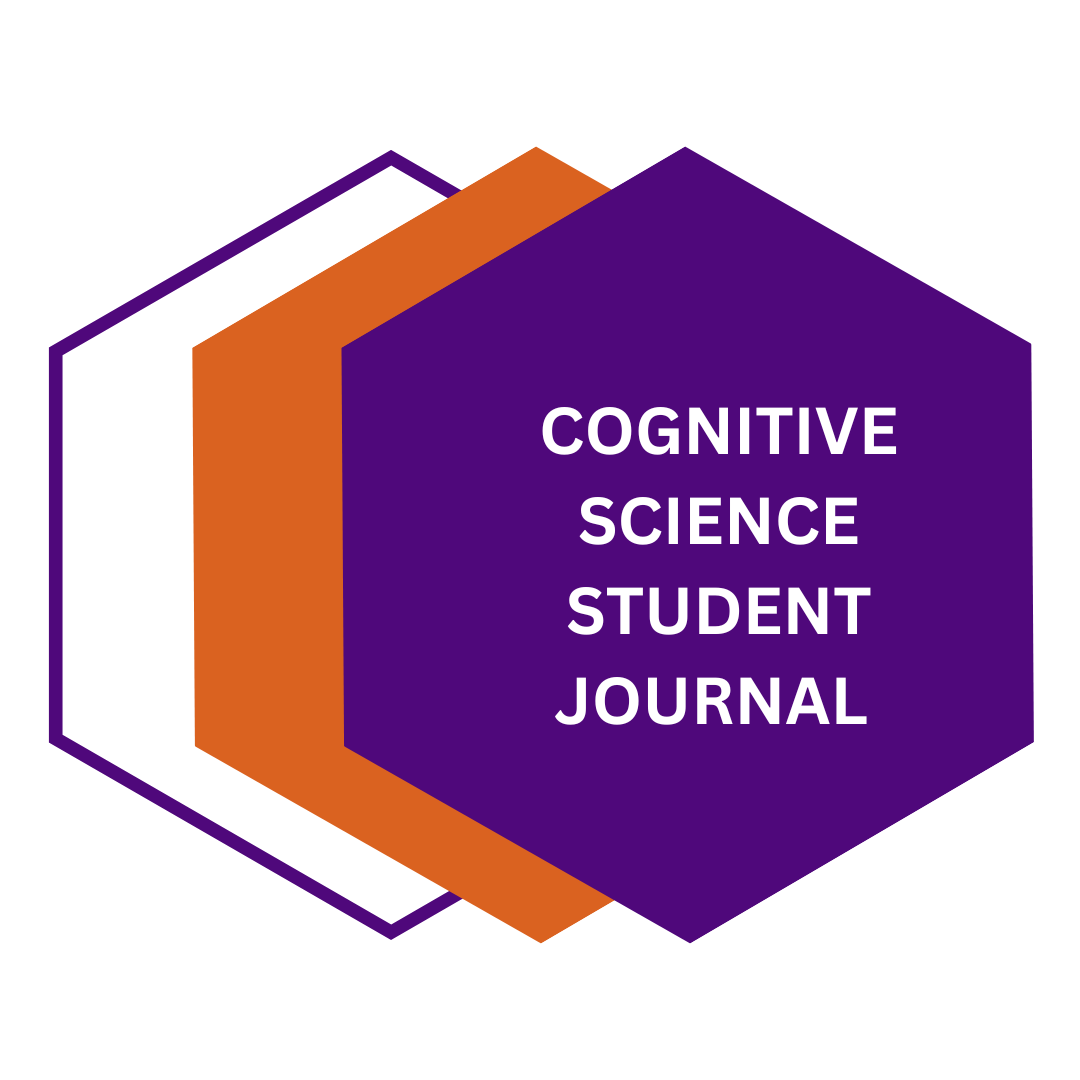
\includegraphics[width=0.6\textwidth]{images/CSSJ_logo.png}
%\end{minipage} 
%\begin{minipage}{0.8\textwidth}
%\Large\textbf{Cognitive Science Student Journal}
%\end{minipage}

%\vspace{2cm}
\begin{tcolorbox}[colback=cssj_purple!80!black,colframe=cssj_purple!80!black]
\color{white}
%\vspace{3cm}
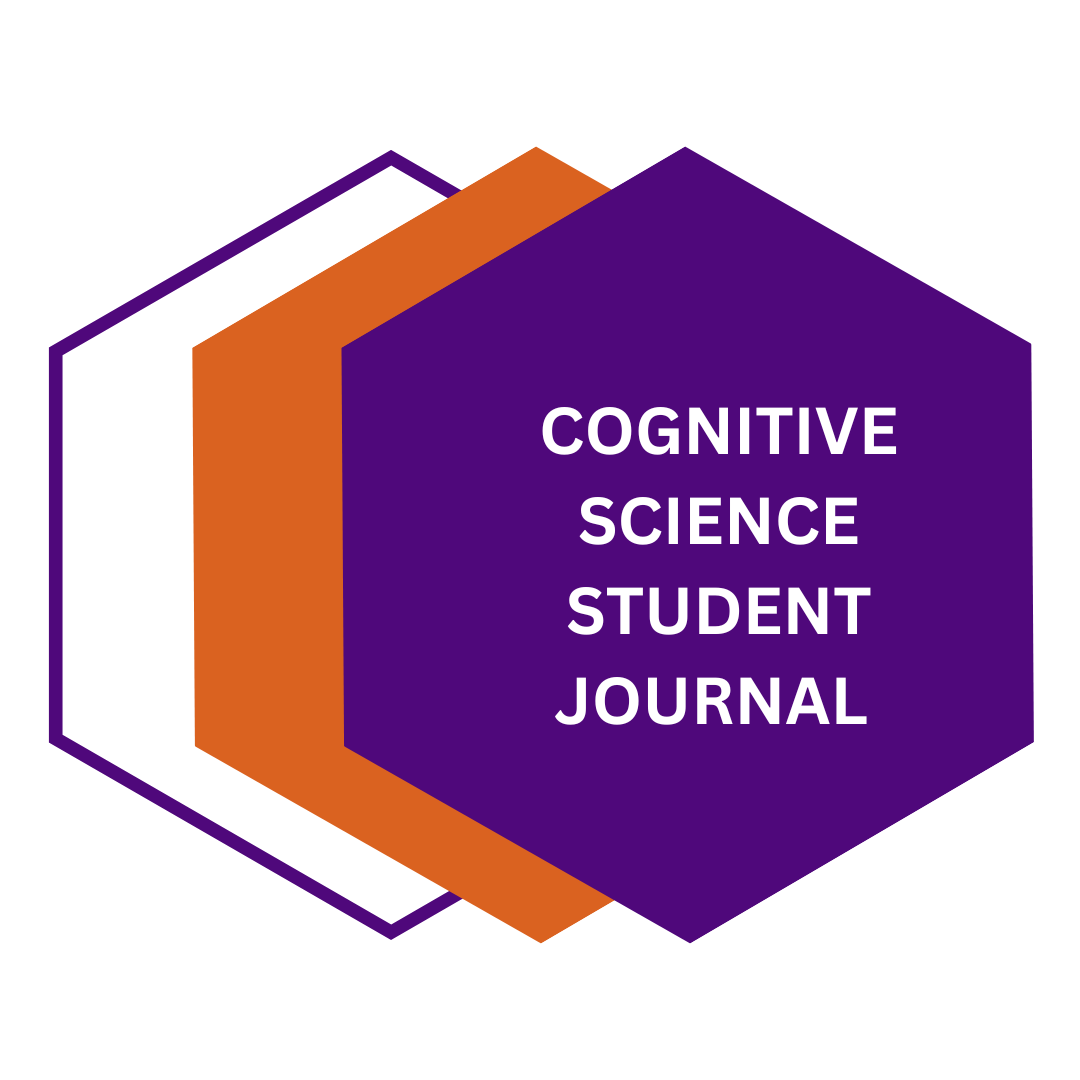
\includegraphics[width=0.3\textwidth]{images/CSSJ_logo.png}

\vspace{1cm}
\noindent \Huge\textbf{Cognitive Science Student Journal Style guide}

\vspace{1cm}
\noindent \huge Complete set of guidelines
\vspace{1cm}
\end{tcolorbox}
    
\vspace{2.5cm}
\noindent The Cognitive Science Student Journal, Osnabrück University, aims at giving its readers an insight into current research and cutting-edge topics at our institute from a student perspective as well as students a platform to publish their work. Its editorial board consists of seminar participants and instructors of the Institute of Cognitive Science at Osnabrück University. 

\vspace{0.6cm}
\noindent The journal can be accessed via: \\
\hyperref[http://cogsci-journal.uni-osnabrueck.de]{\url{http://cogsci-journal.uni-osnabrueck.de}}\\

\noindent Find us on social media: \\
\hyperref[https://www.instagram.com/cogscistudentjournal/]{\url{https://www.instagram.com/cogscistudentjournal/}}\\
\hyperref[https://www.linkedin.com/company/cognitive-science-student-journal/]{\url{https://www.linkedin.com/company/cognitive-science-student-journal/}}\\


\end{titlepage}